\graphicspath{{../../S20_Le_parallelogramme/Images/}}

\themeG
\chapter{Le parallélogramme} \label{S20}

\programme%
   {\item Parallélogramme (une définition et une propriété caractéristique).}
   {\item Mettre en oeuvre ou écrire un protocole de construction d’une figure géométrique.}

\vfill

\begin{debat}{Débat : vocabulaire des quadrilatères}
   Le mot {\bf quadrilatère} provient du latin : {\it quatuor}, quatre, et {\it latus}, côté. Il existe un mot équivalent d'origine grecque : {\bf tétrapleure} de {\it tèssera}, quatre, et {\it pleura}, côté ou {\bf tétragone}, de {\it gônia}, angle. \par
   Comme pour les triangles, les quadrilatères peuvent être particuliers selon qu'ils ont certaines propriétés : parmi ceux-ci, on peut trouver par exemple la famille des trapèzes, des parallélogrammes, des rectangles, des losanges, des carrés ou encore des cerfs-volants.
   \tcblower
      {\psset{unit=0.7}
      \begin{pspicture}(-1,-1)(14,8)
         \psframe[linecolor=red](7.25,0.25)(9.75,7.5)
         \psframe[linecolor=yellow](0.5,0.5)(9.5,2.5)
         \psframe[linecolor=orange](4.25,0)(10,5)
         \psframe[linecolor=orange!50](0.25,-0.25)(10.25,5.25)
         \psframe[linecolor=red!50](0,-0.5)(10.5,7.75)
         \psframe[linecolor=RoyalBlue](-0.25,-0.75)(13.75,8)
         \psset{fillstyle=solid}
         \psframe[fillcolor=yellow](8,1)(9,2) %carré
         \psframe[fillcolor=yellow!50](5,1)(7,2) %rectangle
         \pspolygon[fillcolor=yellow!25](1,1)(3,1)(3,2)(1.5,2) %trapèze rectangle
         \pspolygon[fillcolor=orange!25](1,3.5)(3.5,3.5)(2.5,4.5)(1.5,4.5) %trapèze
         \pspolygon[fillcolor=orange!50](4.5,3.5)(6.25,3.5)(6.75,4.5)(5,4.5) %parallélogramme
         \pspolygon[fillcolor=orange](7.5,4)(8.5,3.5)(9.5,4)(8.5,4.5) %losange
         \pspolygon[fillcolor=red!50](3,6.5)(3,7)(5,7.5)(4.5,6) %convexe
         \pspolygon[fillcolor=red](8,6.75)(8.5,7.25)(9,6.75)(8.5,5.5) %cerf-volant
         \pspolygon[fillcolor=cyan!50](11,1.5)(13.5,3)(13,1.5)(11.25,2.5) %croisé
         \pspolygon[fillcolor=cyan](11,5)(13,5)(12.5,7)(12,5.5) %concave
      \end{pspicture}}
\end{debat}

\hfill {\gray Vidéo : \href{https://www.youtube.com/watch?v=j_seCDgA-lU}{\bf Pourquoi \og mathématiques \fg{} ?}, site Internet {\it m@ths-et-tiques} de {\it Yvan Monka}.}


%%% Approche %%%
\begin{Maquette}[Cours]{Theme={Activité d'approche},Couleur={SteelBlue}}

   \AAtitre{Les bandelettes}

      {\it Objectifs : connaître et reconnaître des figures à quatre côtés ; donner des propriétés de quadrilatères.}

      \begin{AActivite}

         \AApartie{Présentation des bandelettes}     
            Sur les bandelettes représentées ci-dessous, le point O est le milieu des segments [MN] et [PQ] et le point O' est le milieu du segment [RS]. De plus, on a OM = OR.
            \begin{center}
               \small
               \begin{pspicture}(-7,-0.75)(7,0.75)
                  \psframe[linewidth=0.3mm](-6,-0.5)(6,0.5)
                  \psline[linestyle=dashed,linecolor=gray](-6,0)(6,0)
                  \psdot[linewidth=0.4mm](0,0)
                  \rput(0,0.3){O}
                  \psdots[linewidth=0.3mm,linecolor=DodgerBlue](-5,0)(-3,0)(3,0)(5,0)
                  \rput(-5,0.3){\textcolor{DodgerBlue}{M}}
                  \rput(5,0.3){\textcolor{DodgerBlue}{N}}
                  \psdots[linewidth=0.3mm,linecolor=Crimson](-3,0)(3,0)
                  \rput(-3,0.3){\textcolor{Crimson}{P}}
                  \rput(3,0.3){\textcolor{Crimson}{Q}}    
               \end{pspicture} \par
               \begin{pspicture}(-7,-0.5)(7,0.5)
                  \psframe[linewidth=0.3mm](-6,-0.5)(6,0.5)
                  \psline[linestyle=dashed,linecolor=gray](-6,0)(6,0)
                  \psdots[linewidth=0.4mm](0,0)
                  \rput(0.05,0.3){O'}
                  \psdots[linewidth=0.3mm,linecolor=DodgerBlue](-5,0)(5,0)
                  \rput(-5,0.3){\textcolor{DodgerBlue}{R}}
                  \rput(5,0.3){\textcolor{DodgerBlue}{S}}   
               \end{pspicture}
            \end{center}
         
      \AApartie{Construction de quadrilatères}
         \begin{enumerate}
            \item On considère un squelette obtenu en faisant se croiser les deux bandelettes aux points O et O' en plaçant une attache parisienne à travers ces deux points. On s'intéresse aux quadrilatères MRNS tracés à partir de ce squelette.
               \begin{enumerate}
                  \item En plaçant le squelette sur votre feuille, placer les points M, N, R et S puis tracer le quadrilatère MRNS. \par
                     À quelle famille semble appartenir ce quadrilatère ? \pointilles
                  \item Que représentent les segments [MN] et [RS] pour ce quadrilatère ? \pointilles
                  \item Démontrer alors la proposition faite dans la question (a) : \pointilles \par
                     \pointilles 
                  \item Citer d'autres propriétés sur ce quadrilatère particulier. \pointilles \par
                     \pointilles \par
                     \pointilles
                  \item Trouver un cas particulier à cette configuration. \pointilles \par
                     \pointilles
               \end{enumerate}
            \item On s'intéresse maintenant aux quadrilatères PRQS tracés à partir de ce même squelette.
               \begin{enumerate}
                  \item En plaçant le squelette sur votre feuille, placer les points P, Q, R et S puis tracer le quadrilatère PRQS. \par 
                     À quelle famille semble appartenir ce quadrilatère ? \pointilles
                  \item Que représentent les segments [PQ] et [RS] pour ce quadrilatère ? \pointilles
                  \item Conjecturer trois propriétés concernant votre quadrilatère : \pointilles \par
                     \pointilles \par
                     \pointilles
                  \item Trouver un cas particulier à cette configuration. \pointilles \par
                     \pointilles
               \end{enumerate}
         \end{enumerate}

      \end{AActivite}

      \vfill\hfill{\it\footnotesize Source : inspirée du site de \href{http://pernoux.pagesperso-orange.fr/revision/revgeo.pdf}{Dominique Pernoux}}.

\end{Maquette}


%%%Trace écrite %%%
\begin{Maquette}[Cours]{Theme={Trace écrite},Couleur={0.4[SteelBlue,Black]}}

%%%1
\section{Définition et propriétés}

   \begin{definition*}{}
      Un {\bf parallélogramme} est un quadrilatère dont les côtés sont deux à deux parallèles.
   \end{definition*}

   \begin{center}
      {\psset{yunit=0.9}\small
      \begin{pspicture}(0,0.2)(8,4.3)
      \psline[linecolor=DodgerBlue](0.5,0)(2.5,4)
         \psline[linecolor=DodgerBlue](3.5,0.5)(5.5,4.5)
         \psline[linecolor=Crimson](0,1)(5,1.5)
         \psline[linecolor=Crimson](1,3)(6,3.5)
         \rput[rt](0.8,0.95){$A$}
         \rput[lt](4,1.15){$B$}
         \rput[lb](5.25,3.6){$C$}
         \rput[rb](2.1,3.3){$D$}
         \rput(7,2){$\Longrightarrow$}
         \rput(7,2.7){$(AB)//(DC)$}
         \rput(7,1.3){$(AD)//(BC)$}
      \end{pspicture}
      \begin{pspicture}(0,0.2)(6,4.3)
         \pstGeonode[CurveType=polygon,PointSymbol=none,PosAngle={-135,-45,45,135}](1,1){A}(4,1.5){B}(5,3.5){C}(2,3){D}
         \rput(3,2.25){parallélogramme}
      \end{pspicture}}
   \end{center}
  
   Autres caractéristiques d'un parallélogramme : \bigskip

   \begin{tabular}{C{7}C{9.2}}
      {\small \psset{linewidth=0.2mm,unit=1.3}
      \begin{pspicture}(0,0)(3,1.5)
         \pstGeonode[PointSymbol=none,CurveType=polygon,PosAngle={-135,-45,45,135}]{A}(2.5,0.5){B}(3,1.5){C}(0.5,1){D}
         \pstGeonode[PointName=none,PointSymbol=none](1.5,0.75){O}
         \pstLineAB{A}{C}
         \pstLineAB{B}{D}
         \pstSegmentMark[SegmentSymbol=MarkCros,linecolor=DodgerBlue]{O}{A}
         \pstSegmentMark[SegmentSymbol=MarkCros,linecolor=DodgerBlue]{O}{C}
         \pstSegmentMark[linecolor=Crimson]{O}{B}
         \pstSegmentMark[linecolor=Crimson]{O}{D}
      \end{pspicture}}
      &
      \begin{propriete*}{}
         Si un quadrilatère a ses diagonales qui se coupent en leur milieu alors c'est un parallélogramme.
      \end{propriete*} \\
      {\small \psset{linewidth=0.2mm,unit=1.3}
      \begin{pspicture}(0,0)(3,1.5)
         \pstGeonode[PointSymbol=none,CurveType=polygon,PosAngle={-135,-45,45,135}]{A}(2.5,0.5){B}(3,1.5){C}(0.5,1){D}
         \pstGeonode[PointName=none,PointSymbol=none](1.5,0.75){O}
         \pstSegmentMark[SegmentSymbol=MarkCross,linecolor=DodgerBlue]{A}{B}
         \pstSegmentMark[SegmentSymbol=MarkCross,linecolor=DodgerBlue]{D}{C}
         \pstSegmentMark[SegmentSymbol=MarkHash,linecolor=Crimson]{C}{B}
         \pstSegmentMark[SegmentSymbol=MarkHash,linecolor=Crimson]{A}{D}
      \end{pspicture}}
      &
      \begin{propriete*}{}
         Si un quadrilatère a ses côtés opposés de la même longueur deux à deux alors c'est un parallélogramme.
      \end{propriete*} \\
      {\small \psset{linewidth=0.2mm,unit=1.3}
      \begin{pspicture}(0,0)(3,1.5)
         \footnotesize
         \psset{linewidth=0.2mm}
         \pstGeonode[PointSymbol=none,CurveType=polygon,PosAngle={-135,-45,45,135}]{A}(2.5,0.5){B}(3,1.5){C}(0.5,1){D}
         \pstGeonode[PosAngle=90](1.5,0.75){O}
         \pstMarkAngle[linecolor=DodgerBlue]{B}{A}{D}{}
         \pstMarkAngle[linecolor=DodgerBlue]{D}{C}{B}{}
         \pstMarkAngle[linecolor=Crimson,MarkAngleRadius=0.2]{A}{D}{C}{}
         \pstMarkAngle[linecolor=Crimson,MarkAngleRadius=0.3]{A}{D}{C}{}
         \pstMarkAngle[linecolor=Crimson,MarkAngleRadius=0.2]{C}{B}{A}{}
         \pstMarkAngle[linecolor=Crimson,MarkAngleRadius=0.3]{C}{B}{A}{}
      \end{pspicture}}
      &
      \begin{propriete*}{}
         Un parallélogramme possède son centre $O$ comme centre de symétrie. Les angles opposés sont égaux.
      \end{propriete*} \\
   \end{tabular}


%%%2
\section{Parallélogrammes particuliers} %%%

   \begin{center}
      {\small
      \begin{pspicture}(0,1)(16,8)
         \pspolygon(0,3)(3,3)(4,5)(1,5) 
         \psframe(7,5.5)(10,7.5)
         \pspolygon(6.5,1.5)(8.5,0.5)(10.5,1.5)(8.5,2.5)
         \psframe(13.5,2.75)(16,5.25)
         \psline[linestyle=dashed]{->}(3,5.5)(6.5,6.5)
         \rput{18}(4.6,6.3){+ angle $\square$}
         \rput{18}(4.9,5.65){+ diag. =}
         \psline[linestyle=dashed]{->}(3,2.5)(6,1.5)
         \rput{-18}(4.35,1.65){+ long. =}
         \rput{-18}(4.7,2.3){+ diag. $\perp$}
         \psline[linestyle=dashed]{->}(10.5,6.5)(13,5.5)
         \rput{30}(12.2,1.7){+ angle $\square$}
         \rput{30}(11.8,2.25){+ diag. =}
         \psline[linestyle=dashed]{->}(11,1.5)(13,2.5)
         \rput{-20}(11.9,6.3){+ long. =}
         \rput{-20}(11.6,5.7){+ diag. $\perp$}
         \psset{linecolor=Crimson}
            \psline(0,3)(4,5)
            \psline(1,5)(3,3)
            \psline(7,5.5)(10,7.5)
            \psline(7,7.5)(10,5.5)
            \psline(6.5,1.5)(10.5,1.5)
            \psline(8.5,0.5)(8.5,2.5)
            \psline(13.5,5.25)(16,2.75)
            \psline(13.5,2.75)(16,5.25)
         \textcolor{DodgerBlue}{
            \rput(1.5,3){x}
            \rput(2.5,5){x}
            \rput(0.5,4){$\approx$}
            \rput(3.5,4){$\approx$}
            \rput(1.5,4.5){$\circ$}
            \rput(2.5,3.5){$\circ$}
            \rput{30}(1,3.5){|}
            \rput{30}(3,4.5){|}
            \rput(8.5,5.5){x}
            \rput(8.5,7.5){x}
            \rput(7,6.5){$\approx$}
            \rput(10,6.5){$\approx$}
            \rput(7.75,6){$\circ$}
            \rput(7.75,7){$\circ$}
            \rput(9.25,6){$\circ$}
            \rput(9.25,7){$\circ$}
            \rput(13.5,4){x}
            \rput(16,4){x}
            \rput(14.75,2.75){x}
            \rput(14.75,5.25){x}
            \rput(14.125,3.375){$\circ$}
            \rput(15.375,4.625){$\circ$}
            \rput(14.125,4.625){$\circ$}
            \rput(15.375,3.375){$\circ$}
            \rput(7.5,1){x}
            \rput(7.5,2){x}
            \rput(9.5,1){x}
            \rput(9.5,2){x}
            \rput(7.5,1.5){$\circ$}
            \rput(9.5,1.5){$\circ$}
            \rput{90}(8.5,1){|}
            \rput{90}(8.5,2){|}
            \psset{linecolor=RoyalBlue}
            \psframe(7,5.5)(7.3,5.8)
            \psframe(8.5,1.5)(8.8,1.8)
            \psframe(13.5,2.75)(13.8,3.05)
            \pspolygon(14.75,4)(14.95,4.2)(14.75,4.4)(14.55,4.2)}
      \end{pspicture}}
   \end{center}

\end{Maquette}


%%% Exercices %%%
\begin{Maquette}[Fiche,CorrigeFin,Colonnes=2]{}
   
  \begin{multicols}{2}

      \begin{exercice}[SLF] %1
         On considère le parallélogramme $CYAN$ suivant :
         \begin{center}
            \begin{pspicture}(-0.5,-0.25)(5,2.5)
               \small
               \pstGeonode[PointSymbol=none,CurveType=polygon,PosAngle={-135,-45,45,135}]{C}(3.5,0){Y}(4.5,2){A}(1,2){N}
               \pstGeonode[PosAngle=90,PointSymbol=none](2.25,1){O}
               \pstLineAB{Y}{N}
               \pstLineAB{C}{A}
            \end{pspicture}      
         \end{center}
         Coder un maximum d'informations sur la figure.
      \end{exercice}
            
      \begin{Solution}
         \begin{pspicture}(-1,-0.5)(5,2.75)
            {\small
            \pstGeonode[PointSymbol=none,CurveType=polygon,PosAngle={-135,-45,45,135}]{C}(3.5,0){Y}(4.5,2){A}(1,2){N}
            \pstGeonode[PosAngle=90,PointSymbol=none](2.25,1){O}
            \pstLineAB{Y}{N}
            \pstLineAB{C}{A}    
            \pstSegmentMark{C}{Y}
            \pstSegmentMark{N}{A}
            \pstSegmentMark[SegmentSymbol=MarkHash]{N}{C}
            \pstSegmentMark[SegmentSymbol=MarkHash]{Y}{A}
            \pstSegmentMark[SegmentSymbol=MarkCros]{O}{C}
            \pstSegmentMark[SegmentSymbol=MarkCros]{O}{A}
            \pstSegmentMark[SegmentSymbol=MarkArrow]{O}{N}
            \pstSegmentMark[SegmentSymbol=MarkArrow]{Y}{O}
            \psset{linecolor=RoyalBlue}
            \pstMarkAngle{Y}{C}{N}{}
            \pstMarkAngle{N}{A}{Y}{}
            \pstMarkAngle[MarkAngleRadius=0.2]{C}{N}{A}{}
            \pstMarkAngle[MarkAngleRadius=0.3]{C}{N}{A}{}
            \pstMarkAngle[MarkAngleRadius=0.2]{A}{Y}{C}{}
            \pstMarkAngle[MarkAngleRadius=0.3]{A}{Y}{C}{}}
         \end{pspicture}
      \end{Solution}
      
      
      \begin{exercice}[SLF] %2
         Dans les parallélogrammes $ROSE$ et $BLEU$ suivants, compléter toutes les mesures possibles.
         \begin{center}
         {\psset{unit=0.9}
            \begin{pspicture}(0.5,-0.25)(5,2.25)
               \small
               \pspolygon(0,0)(3.5,0)(4.5,2)(1,2) 
               \psline(0,0)(4.5,2)
               \psline(3.5,0)(1,2)
               \rput(-0.2,0){$R$}
               \rput(3.8,0){$O$}
               \rput(4.8,2){$S$}
               \rput(0.7,2){$E$}
               \rput{-38}(3,0.7){\Lg{3}}
               \rput{29}(1.2,0.8){\Lg{4}}
            \end{pspicture}
            \begin{pspicture}(0,-0.25)(3,2.25)
               \footnotesize
               \pspolygon(0,0)(2.5,0)(3.5,2)(1,2) 
               \rput(-0.25,0){$B$}
               \rput(2.8,0){$L$}
               \rput(3.75,2){$E$}
               \rput(0.7,2){$U$}
               \rput(1.4,0.25){\Lg{6}}
               \rput{62}(0.2,1){\Lg{4}}
               \psarc(3.5,2){0.5}{180}{-117}
               \rput(2.7,1.6){63\degre}
               \psarc(1,2){0.5}{-117}{0}
               \rput(1.5,1.4){117\degre}
            \end{pspicture}}
         \end{center}
      \end{exercice}  
      
      \begin{Solution}
         {\psset{unit=0.9} \small
         \begin{pspicture}(5,2.75)
            \pspolygon(0,0)(3.5,0)(4.5,2)(1,2) 
            \psline(0,0)(4.5,2)
            \psline(3.5,0)(1,2)
            \rput(-0.2,0){$R$}
            \rput(3.8,0){$O$}
            \rput(4.8,2){$S$}
            \rput(0.7,2){$E$}
            \rput{-38}(3,0.7){\Lg{3}}
            \rput{24}(1.2,0.8){\Lg{4}}
            \rput{-38}(1.9,1.6){\cor{\Lg{3}}}
            \rput{24}(3,1.6){\cor{\Lg{4}}}
         \end{pspicture}
         \begin{pspicture}(3,2.75)
            \pspolygon(0,0)(2.5,0)(3.5,2)(1,2) 
            \rput(-0.25,0){$B$}
            \rput(2.8,0){$L$}
            \rput(3.75,2){$E$}
            \rput(0.7,2){$U$}
            \rput(1.4,0.25){\Lg{6}}
            \rput{62}(0.2,1){\Lg{4}}
            \rput(2.4,2.25){\cor{\Lg{6}}}
            \rput{62}(3.2,1){\cor{\Lg{4}}}
            \psarc(3.5,2){0.5}{180}{-117}
            \rput(2.7,1.6){\ang{63}}
            \psarc[linecolor=RoyalBlue](2.5,0){0.5}{63}{180}
            \rput(2.2,0.7){\cor{\ang{117}}}
            \psarc[linecolor=RoyalBlue](0,0){0.5}{0}{63}
            \rput(0.7,0.4){\cor{\ang{63}}}
            \psarc(1,2){0.5}{-117}{0}
            \rput(1.5,1.4){\ang{117}}
         \end{pspicture}}
      \end{Solution} 
      
      
      \begin{exercice}[SLF] %3
         Construire sur ce quadrillage les parallélogrammes suivants : $ABCF$, $BCDG$, $CDHE$ et $BIEC$.
         \begin{center}
            {\psset{unit=0.7}
            \begin{pspicture}(11,11)
               \psgrid[subgriddiv=0,gridcolor=lightgray,gridlabels=0](0,0)(11,11)
               \pstGeonode(1,1){A}(5,1){B}(6,3){C}(9,6){D}(3,7){E}         
            \end{pspicture}}
         \end{center} 
      \end{exercice}
      
      \begin{Solution}
         {\psset{unit=0.7}
            \begin{pspicture}(11,11.5)
               \psgrid[subgriddiv=0,gridcolor=lightgray,gridlabels=0](0,0)(11,11)
               \pstGeonode(1,1){A}(5,1){B}(6,3){C}(9,6){D}(3,7){E}
               \pstGeonode[CurveType=polygon,linecolor=DodgerBlue](1,1){A}(5,1){B}(6,3){C}(2,3){F}
               \pstGeonode[CurveType=polygon,linecolor=Crimson](5,1){B}(6,3){C}(9,6){D}(8,4){G}
               \pstGeonode[CurveType=polygon,linecolor=ForestGreen](6,3){C}(9,6){D}(6,10){H}(3,7){E}
               \pstGeonode[CurveType=polygon,linecolor=DarkOrange](5,1){B}(2,5){I}(3,7){E}(6,3){C}
            \end{pspicture}}
      \end{Solution}
      
      
      \begin{exercice} %4
         Construire les parallélogrammes $ABCD$ et $EFGH$.
         \begin{enumerate}
            \item $AB =\Lg{5} \; ; AD =\Lg{3,5}$ et $BD =\Lg{7}$.
            \item $EF =\Lg{2} \; ; EH =\Lg{4,5}$ et $EG = \Lg{3,5}$.
         \end{enumerate}
      \end{exercice}
      
      \begin{Solution}
         \begin{enumerate}
            \item {\small
               \begin{pspicture}(-1.5,1.5)(6,3.8)
                  \pstGeonode[PointSymbol=none,CurveType=polygon,PosAngle={-135,-45,45,135}]{A}(5,0){B}(3.8,3.3){C}(-1.2,3.3){D}
                  \pstLineAB{D}{B}
                  \pstLabelAB{D}{B}{\cor{\Lg{7}}}
                  \pstLabelAB[offset=-3mm]{D}{A}{\cor{\Lg{3,5}}}
                  \pstLabelAB[offset=-3mm]{A}{B}{\cor{\Lg{5}}}
                  \pstSegmentMark[SegmentSymbol=MarkHash]{A}{D}
                  \pstSegmentMark[SegmentSymbol=MarkHash]{B}{C}
                  \pstSegmentMark[SegmentSymbol=MarkCros]{A}{B}
                  \pstSegmentMark[SegmentSymbol=MarkCros]{D}{C}
               \end{pspicture}}
            \item {\small
               \begin{pspicture}(-2,-0.5)(5,4.3)
               \pstGeonode[PointSymbol=none,CurveType=polygon,PosAngle={-135,-45,45,135}]{E}(4.5,0){H}(3.5;25.2){G}(2;131.8){F}
                  \pstLineAB{E}{G}
                  \pstLabelAB{E}{G}{\cor{\Lg{3,5}}}
                  \pstLabelAB[offset=-4mm]{E}{H}{\cor{\Lg{4,5}}}
                  \pstLabelAB[offset=-4mm]{F}{E}{\cor{\Lg{2}}}
                  \pstSegmentMark[SegmentSymbol=MarkCros]{E}{F}
                  \pstSegmentMark[SegmentSymbol=MarkCros]{H}{G}
                  \pstSegmentMark[SegmentSymbol=MarkHashh]{E}{H}
                 \pstSegmentMark[SegmentSymbol=MarkHashh]{F}{G}
            \end{pspicture}}
         \end{enumerate}
      \end{Solution}
      
      
      \begin{exercice} %5
         Construire en vraie grandeur les parallélogrammes schématisés ci-dessous (les longueurs sont en cm).
         {\small
         \begin{colenumerate}
            \item[A] \begin{pspicture}(-0.25,0)(3,2.5)
                  \pstGeonode[PointSymbol=none,PointName=none]{A}(2.5,1){B}(2.5,2.5){C}(0,1.5){D}
                  \pnode(0,0){A}
                  \pnode(2.5,1){B}
                  \pnode(2.5,2.5){C}
                  \pnode(0,1.5){D}
                  \pslineByHand(A)(B)(C)(D)(A)
                  \pstLabelAB{D}{C}{6}
                  \pstLabelAB{A}{D}{4}
                  \pstMarkAngle[LabelSep=0.8]{A}{D}{C}{\ang{110}}
               \end{pspicture}
            \item[B] \begin{pspicture}(-0.25,0)(3,2.7)
                  \pstGeonode[PointSymbol=none,PointName=none]{A}(3,0){B}(2,2){C}(-1,2){D}(1.25,1){O}
                  \pnode(0,0){A}
                  \pnode(3,0){B}
                  \pnode(2.5,2){C}
                  \pnode(-0.5,2){D}
                  \pnode(1.25,1){O}
                  \pslineByHand(A)(B)(C)(D)(A)
                  \pslineByHand(A)(C)
                  \pslineByHand(B)(D)
                  \pstLabelAB[offset=2mm]{D}{O}{3}
                  \pstLabelAB[offset=2mm]{O}{C}{2}
                  \pstMarkAngle[LabelSep=0.8]{D}{O}{A}{\ang{40}}
               \end{pspicture}
            \item[C] \begin{pspicture}(-0.25,0)(3,2)
                  \pstGeonode[PointSymbol=none,PointName=none]{A}(2,0){B}(3,2){C}(1,2){D}
                  \pnode(0,0){A}
                  \pnode(2,0){B}
                  \pnode(3,2){C}
                  \pnode(1,2){D}
                  \pslineByHand(A)(B)(C)(D)(A)
                  \pslineByHand(B)(D)
                  \pstLabelAB[offset=-3mm]{B}{C}{3}
                  \pstLabelAB{D}{C}{5}
                  \pstLabelAB[offset=-3mm]{D}{B}{3,3}
               \end{pspicture}
            \item[D] \begin{pspicture}(0,0)(3,2.7)
                  \pstGeonode[PointSymbol=none,PointName=none]{A}(2.5,0.5){B}(3.5,2.5){C}(1,2){D}(1.75,1.25){O}
                  \pnode(0,0){A}
                  \pnode(2.5,0.5){B}
                  \pnode(3.5,2.5){C}
                  \pnode(1,2){D}
                  \pslineByHand(A)(B)(C)(D)(A)
                  \pslineByHand(A)(C)
                  \pslineByHand(B)(D)
                  \pstLabelAB{A}{D}{2,4}
                  \pstLabelAB[offset=2mm]{A}{O}{2}
                  \pstLabelAB[offset=2mm]{O}{B}{3}
               \end{pspicture}
         \end{colenumerate}}
      \end{exercice}
      
      \begin{Solution}
         \begin{enumerate}
            \item[A] \begin{pspicture}(-0.5,0)(7.4,4)
                  \pstGeonode[PointSymbol=none,CurveType=polygon,PointName=none]{A}(6,0){B}(7.37,3.76){C}(4;70){D}
                  \pstLabelAB{D}{C}{\cor{\Lg{6}}}
                  \pstLabelAB{A}{D}{\cor{\Lg{4}}}
                  \pstMarkAngle{A}{D}{C}{\cor{\ang{110}}}
               \end{pspicture}
            \item[B] \begin{pspicture}(-3.5,-1.5)(3,1.5)
                  \pstGeonode[PointSymbol=none,CurveType=polygon,PointName=none](3;180){A}(2;220){B}(3;0){C}(2;40){D}
                  \pstGeonode[PointSymbol=none,PointName=none]{O}
                  \pstLineAB{A}{C}
                  \pstLineAB{B}{D}
                  \pstLabelAB[offset=-2mm]{O}{D}{\cor{\small \Lg{2}}}
                  \pstLabelAB[offset=2mm]{A}{O}{\cor{\small \Lg{3}}}
                  \pstMarkAngle{A}{O}{B}{\cor{\ang{40}}}
               \end{pspicture}
            \item[C] \begin{pspicture}(-0.5,0)(7,2.5)
                  \pstGeonode[PointSymbol=none,CurveType=polygon,PointName=none]{A}(5,0){B}(7.3,1.9){C}(3;39.6){D}
                  \pstLineAB{B}{D}
                  \pstLabelAB[offset=-3mm]{B}{C}{\cor{\Lg{3}}}
                  \pstLabelAB{D}{C}{\cor{\Lg{5}}}
                  \pstLabelAB[offset=-3mm]{D}{B}{\cor{\Lg{3,3}}}
               \end{pspicture}
            \item[D] \begin{pspicture}(-3.5,-1.5)(3,2)
                  \pstGeonode[PointSymbol=none,CurveType=polygon,PointName=none](3;180){A}(2;232.0){B}(3;0){C}(2;52.9){D}
                  \pstGeonode[PointSymbol=none,PointName=none]{O}
                  \pstLineAB{A}{C}
                  \pstLineAB{B}{D}
                  \pstLabelAB[offset=-3mm]{A}{B}{\cor{\Lg{2,4}}}
                  \pstLabelAB{B}{O}{\cor{\Lg{2}}}
                  \pstLabelAB{O}{C}{\cor{\Lg{3}}}
               \end{pspicture}
            \end{enumerate}

      \end{Solution}
      
      
      \begin{exercice}[Dur] %6
         Construire en vraie grandeur :
         \begin{enumerate}
            \item Un parallélogramme $VERT$ tel que \par
               $VT = \Lg{5} \; ; \widehat{ERT} =\ang{125}$ et $VE =\Lg{4}$.
            \item Un parallélogramme $GRIS$ de centre $O$ tel que \par
               $GR =\Lg{6} \; ; SO =\Lg{3}$ et $IO =\Lg{4}$.
            \item Un parallélogramme $NOIR$ tel que \par
               $NI =\Lg[mm]{62} \; ; \widehat{NIR} =\ang{40}$ et $\widehat{RNI} =\ang{30}$.
         \end{enumerate}
      \end{exercice}
      
      \begin{Solution}
         \begin{enumerate}
            \item \begin{pspicture}(-2.3,-0.3)(6,3.8)
                  \pstGeonode[PointSymbol=none,CurveType=polygon,PosAngle={-135,135,45,-45}]{V}(4;125){E}(2.7,3.3){R}(5,0){T}
                  \pstLabelAB[offset=-3mm]{V}{T}{\cor{\Lg{5}}}
                  \pstLabelAB[offset=-3mm]{E}{V}{\cor{\Lg{4}}}
                  \pstMarkAngle{E}{R}{T}{\cor{\ang{125}}}
               \end{pspicture}
            \item \begin{pspicture}(-1,-0.3)(7,4.5)         
                  \pstGeonode[PointSymbol=none,CurveType=polygon,PosAngle={-135,-45,45,135}]{G}(6,0){R}(8;26.4){I}(1.2,3.6){S}
                  \pstGeonode[PointSymbol=none,PosAngle=90](4;26.4){O}
                  \pstLineAB{G}{I}
                  \pstLineAB{R}{S}
                  \pstLabelAB[offset=-3mm]{G}{R}{\cor{\Lg{6}}}
                  \pstLabelAB{S}{O}{\cor{\Lg{3}}}
                  \pstLabelAB{O}{I}{\cor{\Lg{4}}}
               \end{pspicture}
            \item \begin{pspicture}(-0.5,-2.5)(6.5,2.2)
               \pstGeonode[PointSymbol=none,CurveType=polygon,PosAngle={180,-90,0,90}]{N}(3.35;-40){O}(6.3,0){I}(4.3;30){R}
               \pstLineAB{N}{I}
               \pstLabelAB{N}{I}{\cor{\Lg[mm]{62}}}
               \pstMarkAngle{R}{I}{N}{\cor{\ang{40}}}
               \pstMarkAngle{I}{N}{R}{\cor{\ang{30}}}
            \end{pspicture}
         \end{enumerate}
      \end{Solution}
      
      
      \begin{exercice} %7
         Tracer, puis démontrer\dots
         \begin{enumerate}
            \item Tracer le cercle $(C_1)$ de centre $O$ de rayon \Lg{3,5}.
            \item Placer deux points $N$ et $P$ sur $(C_1)$ tels que [NP] soit un diamètre de $(C_1)$.
            \item Construire le cercle $(C_2)$ de centre $O$ de rayon \Lg{5}.
            \item Placer deux autres points $Q$ et $R$ sur $(C_2)$, non alignés avec $N$ et $P$ tels que $[QR]$ soit un diamètre de $(C_2)$.
            \item Démontrer que le quadrilatère $NQPR$ est un parallélogramme.
            \item Calculer les longueurs $NP$ et $QR$. Justifier.
         \end{enumerate} 
      \end{exercice}
      
      \begin{Solution}
         Questions 1 à 4. \par
         \begin{pspicture}(-5.25,-5.25)(5.25,5.25)
            \pscircle(0,0){3.5}
            \pscircle(0,0){5}
            \psline(3.5;240)(3.5;60)
            \psline(5;190)(5;10)
            \pspolygon[linecolor=RoyalBlue](3.5;240)(5;190)(3.5;60)(5;10)
            \rput(3.8;240){N}
            \rput(5.3;190){Q}
            \rput(3.8;60){P}
            \rput(5.3;10){R}
            \rput(3.9;110){$(C_1)$}
            \rput(5.5;150){$(C_2)$}
            \rput{60}(0.5,1.5){\cor{\Lg{3,5}}}
            \rput{12}(2,0.7){\cor{\Lg{5}}}
            \rput(-0.2,0.4){$O$}
         \end{pspicture}
         \begin{enumerate}
         \setcounter{enumi}{4}
            \item $O$ est le milieu du segment $[QR]$ et également le milieu du segment $[NP]$. \par
            Or, ces deux segments sont les diagonales du quadrilatère $NQPR$ donc, ses diagonales se coupent en leur milieu et par conséquent : \cor{$NQPR$ est un parallélogramme}.
            \item $NP =2OP =2\times\Lg{3,5} =\cor{\Lg{7}}$. \par
               $QR =2OR =2\times\Lg{5} =\cor{\Lg{10}}$.
         \end{enumerate}
      \end{Solution}
      
      
      \begin{exercice}[Dur] %8
         Tracer, puis démontrer\dots{} bis !
         \begin{enumerate}
            \item Tracer un triangle équilatéral $ABC$ de côté \Lg{5}.
            \item À l'extérieur du triangle et de telle sorte que les figures ne se recouvrent pas, placer les points $D$ et $E$ tels que $ABDE$ soit un rectangle avec $AD =\Lg{7}$.
            \item Placer les points $F$ et $G$ tels que $ACFG$ soit un losange avec $\widehat{ACF} =\ang{150}$.
            \item Donner la mesure des angles $\widehat{CAG}$ et $\widehat{BAG}$.
            \item Que peut-on en déduire pour les points $G, A$ et $E$ ?
         \end{enumerate}
      \end{exercice}
      
      \begin{Solution}
         Questions 1 à 3. \par
            \begin{pspicture}(-3,-5.5)(5,9)
               \pstGeonode[PointSymbol=none,PosAngle={180,0,45,-45,-135,45,145}]{A}(5,0){B}(5;60){C}(5,-5){D}(0,-5){E}(2.8,9.5){F}(0,5){G}
               \psset{MarkAngle=90}
               \pstSegmentMark{A}{B}
               \pstSegmentMark{B}{C}
               \pstSegmentMark{A}{C}
               \pstLabelAB{A}{B}{\cor{\Lg{5}}}
               \pstSegmentMark[SegmentSymbol=pstslashhh]{B}{D}
               \pstSegmentMark[SegmentSymbol=pstslashhh]{A}{E}
               \pstSegmentMark{E}{D}
               \pstLabelAB{A}{D}{\cor{\Lg{7}}}
               \pstSegmentMark{C}{F}
               \pstSegmentMark{F}{G}
               \pstSegmentMark{A}{G}
               \pstLineAB{A}{D}
               \pstMarkAngle[Mark=MarkHashhh,MarkAngleRadius=0.5]{F}{C}{A}{\cor{\ang{150}}}
               \pstMarkAngle{B}{A}{C}{\cor{\ang{60}}}
               \pstMarkAngle{C}{B}{A}{\cor{\ang{60}}}
               \pstMarkAngle{A}{C}{B}{\cor{\ang{60}}}
               \pstRightAngle{A}{B}{D}
            \end{pspicture}
         \begin{enumerate}
            \setcounter{enumi}{3}
            \item Le triangle $CAG$ est isocèle en $A$ puisque $AC = AG$ donc, $\widehat{ACG} = \widehat{AGC}$. \par
               De plus, $(GC)$ est un axe de symétrie du losange, donc $\widehat{ACG}=\ang{150}\div2 =\ang{75}$. \par
               La somme des angles dans un triangle vaut \ang{180} donc $\widehat{CAG}+\widehat{AGC}+\widehat{GCA} =\ang{180}$ soit $\widehat{CAG} + \ang{75}+\ang{75}=\ang{180}$ ou encore \cor{$\widehat{CAG} =\ang{30}$}. \par
               $\widehat{BAG} = \widehat{BAC}+\widehat{CAG} =\ang{60}+\ang{30} =\cor{\ang{90}}$.
            \item On a $\widehat{GAE} =\widehat{GAB}+\widehat{BAE} =\ang{90}+\ang{90} =\ang{180}$ donc l'angle $\widehat{GAE}$ est plat d'où : \cor{les points $G, A$ et $E$ sont alignés}.
         \end{enumerate}
      \end{Solution}

   \end{multicols}

\end{Maquette}


%%% Récré %%%
\begin{Maquette}[Cours]{Theme={Activité récréative},Couleur={IndianRed}}
    
   \ARtitre{Les puzzles de Sam Loyd}

      {\it Sam Loyd} (1841-1911) était un mathématicien américain adepte de casse-têtes mathématiques et d'échec. Il est à l'origine de milliers de casse-têtes publiés notamment dans des journaux. On considère l'énigme {\bf The royal road to mathematics}, issu du \og Sam Loyd's cyclopedia of 5000 puzzles tricks and conundrums with answers \fg, page 60.
      \begin{center}
         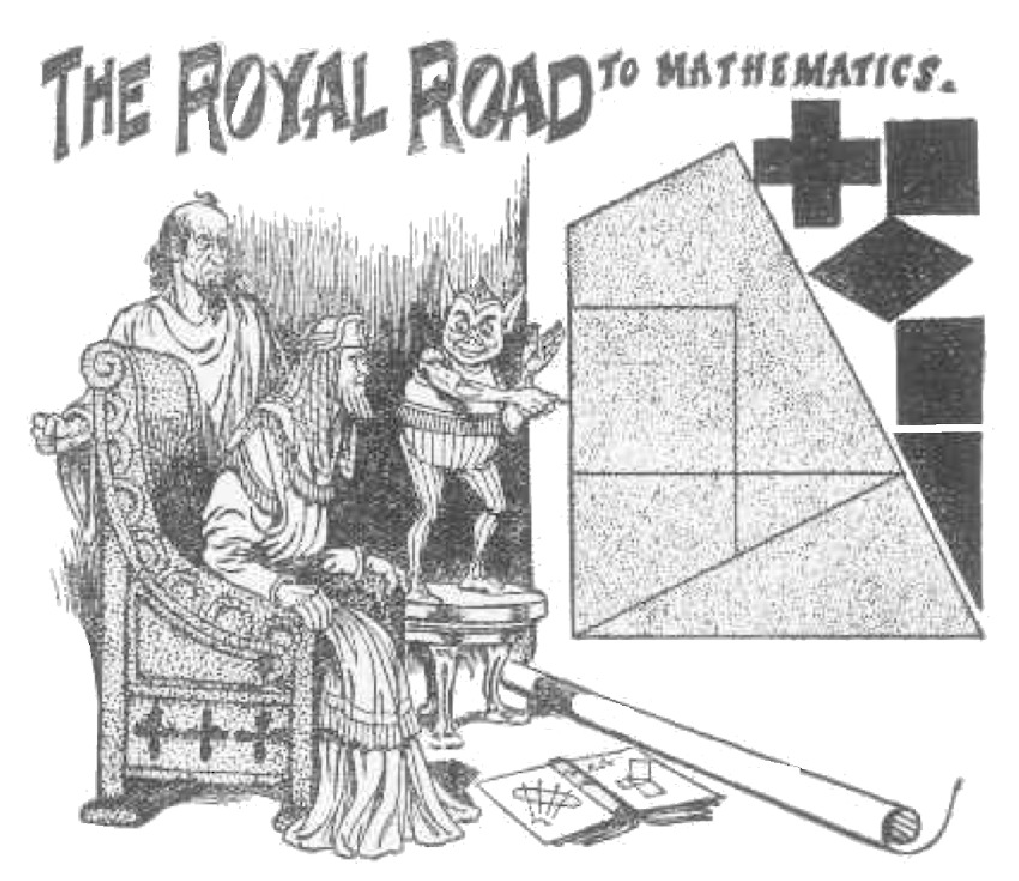
\includegraphics[height=9cm]{Sam_loyd} \quad 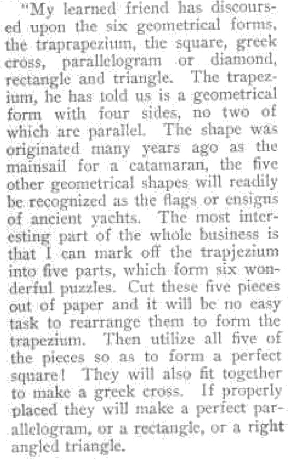
\includegraphics[height=9cm]{Sam_loyd_texte}
      \end{center}

   \begin{multicols}{2}

      \ARpartie{Composition du trapezium}
         On considère le quadrilatère de Sam Loyd \par
         construit sur le quadrillage suivant : \par
            \begin{pspicture}(-1.5,-1.3)(6,7.3)
               \psgrid[subgriddiv=0,gridlabels=0,gridcolor=gray](-1,-1)(6,7)
               \psset{linewidth=0.5mm}
               \pspolygon(0,0)(5,0)(2,6)(0,5)
               \psline(0,0)(4,2)(0,2)
               \psline(0,4)(2,4)(2,1)
               \psline{|-|}(4,5)(4,6)
               \rput(4.5,5.5){\small\Lg{1}}
            \end{pspicture}
            \begin{enumerate}
               \item L'auteur appelle cette figure \og trapezium \fg{} que \par
                  l'on peut traduire par trapèze. Qu'en pensez-vous ? \par
                  Dans le texte, comme définit-il cette figure ?
               \item De quoi est composé ce trapezium ?      
            \end{enumerate}
        
      \ARpartie{Résolution des puzzles}
         Sam Loyd propose, à partir des pièces du trapézium, de reconstituer le carré, la croix grecque, le parallélogramme, le rectangle et le triangle rectangle. \par
         {\psset{unit=0.5}
         \begin{pspicture}(-2,-1)(13,16.5)
            \psset{fillstyle=solid,fillcolor=yellow!30,linewidth=0.8mm}
            \pspolygon(3,0)(13,0)(11,4)
            \pspolygon(0,4)(0,6)(2,6)(2,8)(4,8)(4,6)(6,6)(6,4)(4,4)(4,2)(2,2)(2,4)
            \psframe(8,6)(13,10)
            \pspolygon(2,9)(0,13)(4,15)(6,11)
            \pspolygon(6,15)(11,15)(13,11)(8,11)
            \psgrid[subgriddiv=0,gridlabels=0,gridcolor=gray](-1,-1)(14,16)
            \psline[linewidth=0.5mm]{|-|}(0,0)(0,1)
            \rput(1,0.5){\small\Lg{1}}         
         \end{pspicture}}
         \begin{enumerate}
            \setcounter{enumi}{2}
            \item Reproduire le trapezium puis le découper.
            \item Avec les pièces du puzzle, reconstituer chacune des figures ci-dessus.
         \end{enumerate}
   \end{multicols}

\end{Maquette}